\documentclass[a4paper,11pt]{article}

\usepackage[dutch]{babel}
\usepackage[utf8]{inputenc}
\usepackage{amsmath}
\usepackage{amssymb}
\usepackage{geometry}
\usepackage{enumitem}
\usepackage{graphicx}
\usepackage{tikz}
\usepackage[hidelinks]{hyperref}

\geometry{margin=2.5cm}

\title{Oefeningen Wiskunde voor Systemen}
\author{KU Leuven - ESAT}
\date{\today}

\begin{document}

\maketitle
\tableofcontents
\newpage

\section{Formularium}
\label{sec:formularium}

Dit formularium is een compacte samenvatting van de standaardformules uit het ``Signals and Systems'' formularium. In de oefeningen wordt hiernaar verwezen.

\subsection{Laplace transform (LT)}
\label{form:laplace}

\subsubsection*{1.1 Definitie en eigenschappen}
\label{form:laplace-def}
\label{form:laplace-prop}
\begingroup
\setlength{\tabcolsep}{6pt}
\renewcommand{\arraystretch}{1.35}
\[
\begin{array}{@{}lcl@{}}
\text{Definitie:} & f(t)\,u(t) & \longleftrightarrow\; F(s)=\displaystyle\int_0^{\infty} f(t)e^{-st}\,dt\\
\text{translatie in } s: & f(t)e^{-at}\,u(t) & \longleftrightarrow\; F(s+a)\\
\text{translatie in } t: & f(t-a)\,u(t-a) & \longleftrightarrow\; e^{-as}F(s)\\
\text{afgeleide in } t: & \dfrac{d}{dt}\big(f(t)u(t)\big) & \longleftrightarrow\; sF(s)-f(0^+)\\
 & \dfrac{d^2}{dt^2}\big(f(t)u(t)\big) & \longleftrightarrow\; s^2F(s)-s f(0^+)-f'(0^+)\\

\text{afgeleide in } s: & t\,f(t)\,u(t) & \longleftrightarrow\; -\dfrac{d}{ds}F(s)\\
 & t^n f(t)\,u(t) & \longleftrightarrow\; (-1)^n\,\dfrac{d^n}{ds^n}F(s)\\
\text{convolutie:} & \big(f*g\big)(t)\,u(t) & \longleftrightarrow\; F(s)\,G(s)\\
\text{schaling:} & f(a t) & \longleftrightarrow\; \dfrac{1}{a}\,F\!\left(\dfrac{s}{a}\right)\\
\end{array}
\]
\endgroup

\noindent\textbf{Initial value theorem:}
\[
\lim_{t\to 0^+} f(t)=\lim_{s\to\infty} sF(s).
\]
\noindent\textbf{Final value theorem:}
\[
\lim_{t\to\infty} f(t)=\lim_{s\to 0} sF(s)\quad(\text{onder de gebruikelijke poolvoorwaarden}).
\]
\noindent\textbf{Link met FTC:}
\label{form:lt-ft-link}
\[
\mathrm{LT}(s=j\omega)=\mathrm{FTC}(j\omega)\quad \text{als } x(t) \text{ absoluut integreerbaar is.}
\]

\subsubsection*{1.2 Useful Laplace pairs}
\label{form:laplace-pairs}
\begingroup
\setlength{\tabcolsep}{10pt}
\renewcommand{\arraystretch}{1.35}
\[
\begin{array}{@{}lcl@{\qquad}lcl@{}}
e^{-at}u(t) & \longleftrightarrow & \dfrac{1}{s+a} & t^n u(t) & \longleftrightarrow & \dfrac{n!}{s^{n+1}}\\
\cos(a t)u(t) & \longleftrightarrow & \dfrac{s}{s^2+a^2} & \sin(a t)u(t) & \longleftrightarrow & \dfrac{a}{s^2+a^2}\\
\delta(t) & \longleftrightarrow & 1 & u(t) & \longleftrightarrow & \dfrac{1}{s}\\
t\cos(a t)u(t) & \longleftrightarrow & \dfrac{s^2-a^2}{(s^2+a^2)^2} & t\sin(a t)u(t) & \longleftrightarrow & \dfrac{2sa}{(s^2+a^2)^2}
\end{array}
\]
\endgroup

\subsection{Fourier transform (FTC)}
\label{form:ft}

\subsubsection*{2.1 Basic formulae}
\label{form:ft-def}
\label{form:ft-prop}
\[
X(\omega)=\int_{-\infty}^{\infty} x(t)e^{-j\omega t}\,dt,\qquad
x(t)=\frac{1}{2\pi}\int_{-\infty}^{\infty} X(\omega)e^{j\omega t}\,d\omega.
\]

\begingroup
\setlength{\tabcolsep}{6pt}
\renewcommand{\arraystretch}{1.35}
\[
\begin{array}{@{}lcl@{}}
\text{convolution theorem (tijd):} & f(t)*g(t) & \longleftrightarrow\; F(\omega)\,G(\omega)\\
\text{convolution theorem (freq.):} & f(t)\,g(t) & \longleftrightarrow\; \dfrac{1}{2\pi}\,(F*G)(\omega)\\
\text{translatie:} & x(t-t_0) & \longleftrightarrow\; X(\omega)e^{-j\omega t_0}\\
\text{symmetry (reëel $x$):} &  & X(-\omega)=X^*(\omega)\\
\text{time symmetry (reëel $x$):} & x(-t) & \longleftrightarrow\; X(-\omega)=X^*(\omega)\\
\text{link FS--FTC:} &  & X(k\omega_0)=T\,c_k\quad(\omega_0=2\pi/T)
\end{array}
\]
\endgroup

\subsubsection*{2.2 Useful Fourier pairs}
\label{form:ft-pairs}
We gebruiken $\mathrm{sinc}(x)=\dfrac{\sin(x)}{x}$.

\begingroup
\setlength{\tabcolsep}{8pt}
\renewcommand{\arraystretch}{1.4}
\[
\begin{array}{@{}lcl@{}}
\text{Block:} & x(t)=\begin{cases}A,& t\in[-L/2,L/2]\\0,& \text{elders}\end{cases}
& \longleftrightarrow\; X(\omega)=AL\,\mathrm{sinc}\!\left(\dfrac{\omega L}{2}\right)\\
\text{Sinc:} & x(t)=A\,\mathrm{sinc}(\omega_0 t)
& \longleftrightarrow\; X(\omega)=\begin{cases}\dfrac{A\pi}{\omega_0},& |\omega|<\omega_0\\0,& \text{elders}\end{cases}\\
\text{Impuls:} & \delta(t-t_0) & \longleftrightarrow\; e^{-j\omega t_0}\\
\text{Complex expon.:} & e^{j\omega_0 t} & \longleftrightarrow\; 2\pi\,\delta(\omega-\omega_0)\\
\text{Cosine:} & \cos(\omega_0 t) & \longleftrightarrow\; \pi\,[\delta(\omega+\omega_0)+\delta(\omega-\omega_0)]\\
\text{Sine:} & \sin(\omega_0 t) & \longleftrightarrow\; j\pi\,[\delta(\omega+\omega_0)-\delta(\omega-\omega_0)]\\
\text{Delta train:} & \sum\limits_{k=-\infty}^{\infty}\delta(t-kT) & \longleftrightarrow\; \dfrac{2\pi}{T}\sum\limits_{k=-\infty}^{\infty}\delta\!\left(\omega-\dfrac{2\pi k}{T}\right)
\end{array}
\]
\endgroup

\subsection{Fourier series (FS)}
\label{form:fs}

\subsubsection*{3.1 Cartesian form}
\label{form:fs-cart}
Voor periode $T$ met $\omega_0=\dfrac{2\pi}{T}$:
\[
f(t)=\frac{a_0}{2}+\sum_{k=1}^{\infty}\left[a_k\cos\left(\frac{2\pi k}{T}t\right)+b_k\sin\left(\frac{2\pi k}{T}t\right)\right].
\]
\[
a_0=\frac{2}{T}\int_{0}^{T} f(t)\,dt,\qquad
a_k=\frac{2}{T}\int_{0}^{T} f(t)\cos\left(\frac{2\pi k}{T}t\right)\,dt,\qquad
b_k=\frac{2}{T}\int_{0}^{T} f(t)\sin\left(\frac{2\pi k}{T}t\right)\,dt.
\]

\subsubsection*{3.2 Complex form}
\label{form:fs-cplx}
\[
x(t)=\sum_{k=-\infty}^{\infty} c_k e^{jk\omega_0 t},\qquad \omega_0=\frac{2\pi}{T},\qquad
c_k=\frac{1}{T}\int_{0}^{T} f(t)\,e^{-jk\omega_0 t}\,dt.
\]
\noindent\textbf{symmetry (reëel $f$):}\; $c_{-k}=c_k^*$.

\noindent\textbf{Spectrum:}
\[
X(\omega)=\frac{2\pi}{T}\sum_{k=-\infty}^{\infty} c_k\,\delta(\omega-k\omega_0).
\]

\subsubsection*{3.3 Links between cartesian and complex form}
\label{form:fs-ft-link}
\[
c_k=\frac{a_k-jb_k}{2},\qquad c_k^*=\frac{a_k+jb_k}{2}.
\]
\[
|c_k|=\frac{1}{2}\sqrt{a_k^2+b_k^2},\qquad \varphi_k=\mathrm{Arctan2}(a_k,-b_k).
\]
\[
a_k=2\,\mathrm{Re}\{c_k\},\qquad b_k=-2\,\mathrm{Im}\{c_k\}.
\]

\newpage

\section{Hoofdstuk 1: Signalen en Systemen - Eerste Kennismaking}

\subsection{Oefening 1.1: Lineaire Systemen}

Gegeven een systeem met operator $\mathcal{T}$ gedefinieerd als $\mathcal{T}\{x(t)\} = 3x(t) + 2$.

\textbf{Vraag:} Onderzoek of dit systeem lineair is.

\subsection{Oefening 1.2: RC-Circuit}

Een RC-circuit heeft $R = 1000$ $\Omega$ en $C = 10$ $\mu$F. De ingangsspanning is een stapfunctie $v_{\text{in}}(t) = 5u(t)$ V.

\textbf{Vraag:}
\begin{enumerate}[label=(\alph*)]
\item Schrijf de differentiaalvergelijking op voor de uitgangsspanning $v_{\text{uit}}(t)$.
\item Bereken de tijdsconstante $\tau$ van het circuit.
\item Bepaal de uitgangsspanning na $10$ ms als $v_{\text{uit}}(0) = 0$ V.
\end{enumerate}

\subsection{Oefening 1.3: Radioactief Verval}

Een radio-isotoop heeft een halveringstijd van $6$ uur. Om 08:00 uur wordt 20 mg geproduceerd.

\textbf{Vraag:} Hoeveel milligram blijft over om 14:00 uur?

\subsection{Oefening 1.4: Homogeniteit en Additiviteit}

Gegeven twee systemen:
\begin{itemize}
\item Systeem A: $\mathcal{T}\{x(t)\} = 2x(t)$
\item Systeem B: $\mathcal{T}\{x(t)\} = x(t) + 1$
\end{itemize}

\textbf{Vraag:}
\begin{enumerate}[label=(\alph*)]
\item Test beide systemen op homogeniteit (schaling): $\mathcal{T}\{ax(t)\} = a\mathcal{T}\{x(t)\}$.
\item Test beide systemen op additiviteit: $\mathcal{T}\{x_1(t) + x_2(t)\} = \mathcal{T}\{x_1(t)\} + \mathcal{T}\{x_2(t)\}$.
\item Bepaal voor elk systeem of het lineair is.
\end{enumerate}

\subsection{Oefening 1.5: LTI-Systeem Herkenning}

Welke van de volgende systemen zijn lineair en tijdinvariant (LTI)?

\begin{enumerate}[label=(\alph*)]
\item $y(t) = x(t-2)$
\item $y(t) = tx(t)$
\item $y(t) = |x(t)|$
\item $y(t) = \int_0^t x(\tau) d\tau$
\end{enumerate}

\textbf{Vraag:} Motiveer je antwoorden.

\subsection{Oefening 1.6: Causaliteit en Invertibiliteit}

Gegeven het systeem $\mathcal{T}$ met
\[
y(t) = \mathcal{T}\{x(t)\} = x(t) + x(t-1).
\]

\textbf{Vraag:}
\begin{enumerate}[label=(\alph*)]
\item Is het systeem lineair en tijdinvariant?
\item Is het systeem causaal?
\item Is het systeem invertibel? Motiveer.
\end{enumerate}

\subsection{Oefening 1.7: Snelle check (lineariteit, TI en causaliteit)}

Beschouw de twee systemen:
\[
	\text{(S1)}\; y(t)=2x(t-1),\qquad \text{(S2)}\; y(t)=x(t)+u(t).
\]

\textbf{Vraag:}
\begin{enumerate}[label=(\alph*)]
\item Onderzoek voor (S1) en (S2) of het systeem lineair is.
\item Onderzoek voor (S1) en (S2) of het systeem tijdinvariant is.
\item Is elk systeem causaal? Motiveer kort.
\end{enumerate}

\newpage

\section{Hoofdstuk 2: Basissignalen en Bewerkingen}

\subsection{Oefening 2.1: Exponentiële Functies}

Gegeven de signalen $x_1(t) = e^{0.2t}$ en $x_2(t) = e^{-0.5t}$.

\textbf{Vraag:}
\begin{enumerate}[label=(\alph*)]
\item Bepaal welk signaal exponentiële groei en welk exponentieel verval vertoont.
\item Bereken de waarde van elk signaal op $t = 5$ s.
\end{enumerate}

\subsection{Oefening 2.2: Sinus en Cosinus}

Een sinusgolf is gegeven door $x(t) = 3\sin(4\pi t + \frac{\pi}{6})$.

\textbf{Vraag:}
\begin{enumerate}[label=(\alph*)]
\item Bepaal de amplitude, hoekfrequentie $\omega$, frequentie $f$, en fasehoek.
\item Schrijf dit signaal als een cosinusfunctie.
\end{enumerate}

\subsection{Oefening 2.3: Complexe Exponentiële Functie}

Gegeven $z(t) = e^{j2\pi t}$.

\textbf{Vraag:}
\begin{enumerate}[label=(\alph*)]
\item Schrijf dit signaal in termen van sinus en cosinus gebruikmakend van de formule van Euler.
\item Bepaal de waarde op $t = 0.25$ s.
\end{enumerate}

\subsection{Oefening 2.4: Convolutie}

Bereken de convolutie van twee pulssignalen:
\[
f(t) = u(t) - u(t-1), \quad g(t) = u(t) - u(t-1)
\]

\begin{center}
\begin{tikzpicture}[x=1.2cm,y=1.2cm]
\draw[->] (-0.5,0) -- (3.2,0) node[right] {$t$};
\draw[->] (0,-0.2) -- (0,1.6) node[above] {};
\node[below left] at (0,0) {0};

% f(t) and g(t) (identical)
\draw[thick] (0,0) -- (0,1) -- (1,1) -- (1,0);
\node[above] at (0.5,1) {$f(t)=g(t)$};
\node[below] at (1,0) {1};
\end{tikzpicture}
\end{center}

\emph{Zie Formularium: convolutie in tijd $\leftrightarrow$ product in frequentie in \ref{form:ft-prop}.}

\textbf{Vraag:} Bepaal $(f * g)(t)$ en schets het resultaat.

\subsection{Oefening 2.5: Signaalverschuiving en Schaling}

Gegeven het signaal $x(t) = e^{-t}u(t)$.

\begin{center}
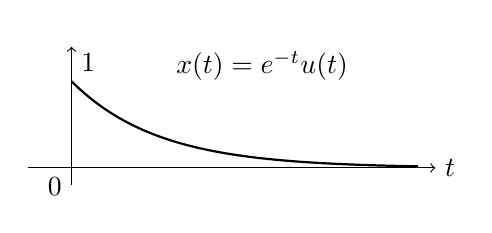
\begin{tikzpicture}[x=1.1cm,y=1.1cm]
\draw[->] (-0.5,0) -- (4.2,0) node[right] {$t$};
\draw[->] (0,-0.2) -- (0,1.4) node[above] {};
\node[below left] at (0,0) {0};
\draw[thick,domain=0:4,samples=60] plot (\x,{exp(-\x)});
\draw[dashed] (0,1) -- (0,0) node[below left] {};
\node[above right] at (0,1) {$1$};
\node[above] at (2.2,0.9) {$x(t)=e^{-t}u(t)$};
\end{tikzpicture}
\end{center}

\textbf{Vraag:}
\begin{enumerate}[label=(\alph*)]
\item Bepaal $y_1(t) = x(t-2)$ (tijdsverschuiving).
\item Bepaal $y_2(t) = x(2t)$ (tijdscompressie).
\item Bepaal $y_3(t) = 2x(t)$ (amplitude schaling).
\item Schets alle drie signalen.
\end{enumerate}

\subsection{Oefening 2.6: Signaalenergie}

Bepaal de energie van de volgende signalen:

\textbf{Vraag:}
\begin{enumerate}[label=(\alph*)]
\item $x(t) = e^{-t}u(t)$
\item $x(t) = 2\sin(t)u(t)$ over $0 \le t \le \pi$
\item $x(t) = \text{rect}(t) = u(t+0.5) - u(t-0.5)$
\end{enumerate}

\subsection{Oefening 2.7: Driehoeksignaal met Stapfuncties}

Definieer het signaal
\[
x(t) = t\big(u(t)-u(t-1)\big) + (2-t)\big(u(t-1)-u(t-2)\big).
\]

\begin{center}
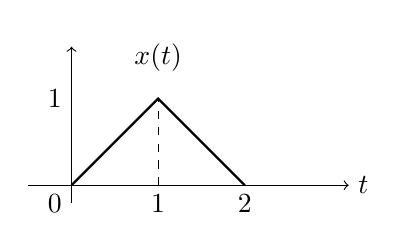
\begin{tikzpicture}[x=1.1cm,y=1.1cm]
\draw[->] (-0.5,0) -- (3.2,0) node[right] {$t$};
\draw[->] (0,-0.2) -- (0,1.6) node[above] {};
\node[below left] at (0,0) {0};
\draw[thick] (0,0) -- (1,1) -- (2,0);
\draw[dashed] (1,0) -- (1,1);
\node[below] at (1,0) {1};
\node[below] at (2,0) {2};
\node[left] at (0,1) {1};
\node[above] at (1,1.2) {$x(t)$};
\end{tikzpicture}
\end{center}

\textbf{Vraag:}
\begin{enumerate}[label=(\alph*)]
\item Schrijf $x(t)$ expliciet als stukgewijze functie.
\item Bereken de energie $E = \int_{-\infty}^{\infty} |x(t)|^2\,dt$.
\item Bepaal en schets $x(t-1)$.
\end{enumerate}

\subsection{Oefening 2.8: Basis signaalbewerkingen (stapfunctie)}

Neem
\[
x(t)=u(t)-u(t-2).
\]

\textbf{Vraag:}
\begin{enumerate}[label=(\alph*)]
\item Schets $x(t)$.
\item Schrijf $x(t-1)$ en $x(t+1)$ in termen van stapfuncties en schets ze.
\item Schrijf $x(2t)$ en $x(-t)$ in termen van stapfuncties en schets ze.
\end{enumerate}

\newpage

\section{Hoofdstuk 3: Laplacetransformatie}

\subsection{Oefening 3.1: Eenvoudige Laplacetransformaties}

Bepaal de Laplacetransformatie van de volgende functies:

\emph{Zie Formularium: definitie \ref{form:laplace-def} en paren \ref{form:laplace-pairs}.}

\textbf{Vraag:}
\begin{enumerate}[label=(\alph*)]
\item $f(t) = 5u(t)$
\item $f(t) = e^{-3t}u(t)$
\item $f(t) = t \cdot u(t)$
\item $f(t) = \cos(5t) \cdot u(t)$
\end{enumerate}

\subsection{Oefening 3.2: Inverse Laplacetransformatie}

Bepaal de inverse Laplacetransformatie van:
\[
F(s) = \frac{3}{s+2} + \frac{5}{s^2 + 4}
\]

\textbf{Vraag:} Vind $f(t)$.

\emph{Zie Formularium: paren \ref{form:laplace-pairs}.}

\subsection{Oefening 3.3: Eerste-Orde Systeem}

Los de volgende differentiaalvergelijking op met Laplacetransformatie:
\[
\frac{dy}{dt} + 4y = 8u(t), \quad y(0) = 2
\]

\textbf{Vraag:} Bepaal $y(t)$.

\emph{Zie Formularium: afgeleide-eigenschap \ref{form:laplace-prop}.}

\subsection{Oefening 3.4: Tweede-Orde Systeem}

Een massa-veer-dempersysteem wordt beschreven door:
\[
\frac{d^2y}{dt^2} + 4\frac{dy}{dt} + 3y = 0, \quad y(0) = 1, \quad y'(0) = 0
\]

\textbf{Vraag:}
\begin{enumerate}[label=(\alph*)]
\item Bepaal de karakteristieke vergelijking.
\item Vind de wortels van de karakteristieke vergelijking.
\item Los de differentiaalvergelijking op voor $y(t)$.
\end{enumerate}

\subsection{Oefening 3.5: Laplace-transformatie met Verschuiving}

Gegeven $F(s) = \frac{2}{s^2 + 4}$.

\textbf{Vraag:}
\begin{enumerate}[label=(\alph*)]
\item Bepaal $f(t) = \mathcal{L}^{-1}\{F(s)\}$.
\item Bepaal $g(t) = \mathcal{L}^{-1}\{e^{-2s}F(s)\}$ gebruikmakend van de tijdsverschuivingsstelling.
\end{enumerate}

\emph{Zie Formularium: tijdsverschuiving in $t$ \ref{form:laplace-prop}.}

\subsection{Oefening 3.6: Partieelbreuken}

Bepaal de inverse Laplacetransformatie van:
\[
F(s) = \frac{10}{(s+1)(s+2)(s+3)}
\]

\textbf{Vraag:} Bepaal $f(t)$ via partieelbreukontwikkeling.

\subsection{Oefening 3.7: Begin- en Eindwaardestelling}

Gegeven de functie in het s-domein:
\[
F(s) = \frac{3s + 5}{s^2 + 4s + 3}
\]

\textbf{Vraag:}
\begin{enumerate}[label=(\alph*)]
\item Bepaal de beginwaarde $f(0^+)$ met de beginwaardestelling.
\item Bepaal de eindwaarde $f(\infty)$ met de eindwaardestelling.
\item Controleer je antwoorden door $f(t)$ te berekenen.
\end{enumerate}

\emph{Zie Formularium: begin- en eindwaardestelling \ref{form:laplace-prop}.}

\subsection{Oefening 3.8: Convolutie via Laplace}

Gegeven
\[
f(t) = u(t) - u(t-1), \quad g(t) = e^{-2t}u(t).
\]
Definieer $y(t) = (f*g)(t)$.

\emph{Zie Formularium: convolutie-eigenschap \ref{form:laplace-prop}.}

\textbf{Vraag:}
\begin{enumerate}[label=(\alph*)]
\item Bepaal $F(s)$ en $G(s)$.
\item Gebruik de convolutie-eigenschap in het $s$-domein om $Y(s)$ te vinden.
\item Bepaal $y(t)$ en geef het antwoord stukgewijs.
\end{enumerate}

\subsection{Oefening 3.9: Laplace}

\textbf{Vraag:}
\begin{enumerate}[label=(\alph*)]
\item Bepaal $\mathcal{L}\{u(t)\}$.
\item Bepaal $\mathcal{L}\{e^{-2t}u(t)\}$.
\item Bepaal $\mathcal{L}\{t\,u(t)\}$.
\item Bepaal de inverse Laplace van $\displaystyle F(s)=\frac{1}{s+3}+\frac{2}{s^2}$.
\end{enumerate}

\newpage

\section{Hoofdstuk 4: Fouriertransformatie}

\subsection{Oefening 4.1: Fouriertransformatie van Rechthoekpuls}

Gegeven een rechthoekpuls:
\[
f(t) = \begin{cases}
A, & -T/2 < t < T/2 \\
0, & \text{elsewhere}
\end{cases}
\]

\begin{center}
\begin{tikzpicture}[x=1.2cm,y=1.2cm]
\draw[->] (-2.8,0) -- (2.8,0) node[right] {$t$};
\draw[->] (0,-0.2) -- (0,1.8) node[above] {};
\node[below left] at (0,0) {0};
\draw[thick] (-1.5,0) -- (-1.5,1.2) -- (1.5,1.2) -- (1.5,0);
\node[above] at (0,1.2) {$A$};
\node[below] at (-1.5,0) {$-T/2$};
\node[below] at (1.5,0) {$T/2$};
\end{tikzpicture}
\end{center}

\emph{Zie Formularium: blok $\leftrightarrow$ sinc in \ref{form:ft-pairs}.}

\textbf{Vraag:}
\begin{enumerate}[label=(\alph*)]
\item Bepaal de Fouriertransformatie $F(j\omega)$.
\item Schrijf het resultaat in de vorm van een sinc-functie.
\item Bepaal de eerste nulpunten van het spectrum.
\end{enumerate}

\subsection{Oefening 4.2: Verschuivingsstelling}

Gegeven $F\{f(t)\} = F(j\omega)$ bepaal de Fouriertransformatie van $f(t-t_0)$.

\emph{Zie Formularium: tijdverschuiving \ref{form:ft-prop}.}

\textbf{Vraag:}
\begin{enumerate}[label=(\alph*)]
\item Geef het bewijs van de verschuivingsstelling.
\item Pas deze toe op de puls uit oefening 4.1 met $t_0 = 1$ s, $A = 2$, $T = 2$ s.
\item Bespreek het effect op amplitude- en fasespectrum.
\end{enumerate}

\subsection{Oefening 4.3: Modulation Property}

Bepaal de Fouriertransformatie van het gemoduleerde signaal:
\[
x(t) = \cos(10\pi t) \cdot \text{rect}(t)
\]

waarbij $\text{rect}(t) = u(t+1) - u(t-1)$ is.

\emph{Zie Formularium: modulatie (cosinus) in \ref{form:ft-pairs}.}

\textbf{Vraag:}
\begin{enumerate}[label=(\alph*)]
\item Pas de modulatiestelling toe.
\item Schets het amplitude- en fasespectrum.
\end{enumerate}

\subsection{Oefening 4.4: Parseval's Stelling}

De energiedichtheid van een signaal wordt gegeven door Parseval's stelling. Gegeven $f(t) = e^{-t}u(t)$.

\emph{Zie Formularium: FTC-definitie \ref{form:ft-def} en eigenschappen \ref{form:ft-prop}.}

\textbf{Vraag:}
\begin{enumerate}[label=(\alph*)]
\item Bepaal de totale energie in het tijdsdomein: $E = \int_{-\infty}^{\infty} |f(t)|^2 dt$.
\item Bepaal $F(j\omega)$ en controleer de energie in het frequentiedomein.
\item Verifieer Parseval's stelling.
\end{enumerate}

\subsection{Oefening 4.5: Exponentieel Signaal}

Gegeven $f(t) = e^{-a|t|}$ met $a > 0$.

\textbf{Vraag:}
\begin{enumerate}[label=(\alph*)]
\item Bepaal de Fouriertransformatie $F(j\omega)$.
\item Schets het amplitude- en fasespectrum.
\item Bepaal de bandbreedte (eerste nulpunt).
\end{enumerate}

\subsection{Oefening 4.6: Dirac Delta}

Bepaal de Fouriertransformatie van:

\textbf{Vraag:}
\begin{enumerate}[label=(\alph*)]
\item $f(t) = \delta(t)$ (impulsfunctie)
\item $f(t) = \delta(t-t_0)$ (verschoven impulsfunctie)
\item $f(t) = \cos(\omega_0 t)$ (hint: gebruik dat $\cos(\omega_0 t) = \frac{1}{2}(e^{j\omega_0 t} + e^{-j\omega_0 t})$)
\end{enumerate}

\subsection{Oefening 4.7: Verschuiving in de Tijd (FTC)}

Beschouw het bloksignaal
\[
x(t) = \begin{cases}
2, & -\tfrac{1}{2} < t < \tfrac{1}{2}\\
0, & \text{elsewhere}
\end{cases}
\]
en definieer $y(t) = x(t-t_0)$ met $t_0 = \tfrac{1}{4}$.

\textbf{Vraag:}
\begin{enumerate}[label=(\alph*)]
\item Bepaal $X(j\omega)$.
\item Bepaal $Y(j\omega)$ met de verschuivingsstelling en bespreek het effect op fase en amplitude.
\end{enumerate}

\subsection{Oefening 4.8: FTC van delta's}

Gebruik de bekende paren $\mathcal{F}\{\delta(t)\}=1$ en de verschuivingsstelling.

\textbf{Vraag:}
\begin{enumerate}[label=(\alph*)]
\item Bepaal $\mathcal{F}\{\delta(t-t_0)\}$.
\item Bepaal de Fouriertransformatie van $x(t)=2\delta(t)-\delta(t-1)$.
\item Wat is het amplitudespectrum van $x(t)$ uit (b)? (geen volledige schets nodig)
\end{enumerate}

\newpage

\section{Hoofdstuk 5: Fourierreeksen}

\subsection{Oefening 5.1: Blokgolf}

Een periodieke blokgolf met periode $T = 2$ s is gedefinieerd als:
\[
f(t) = \begin{cases}
1, & 0 < t < 1 \\
-1, & 1 < t < 2
\end{cases}
\]

\begin{center}
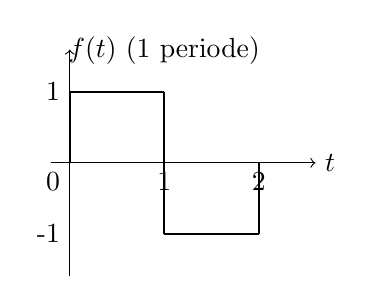
\begin{tikzpicture}[x=1.2cm,y=0.9cm]
\draw[->] (-0.2,0) -- (2.6,0) node[right] {$t$};
\draw[->] (0,-1.6) -- (0,1.6) node[above] {};
\node[below left] at (0,0) {0};
\draw[thick] (0,1) -- (1,1);
\draw[thick] (1,-1) -- (2,-1);
\draw[thick] (0,1) -- (0,0);
\draw[thick] (1,1) -- (1,-1);
\draw[thick] (2,-1) -- (2,0);
\node[below] at (1,0) {1};
\node[below] at (2,0) {2};
\node[left] at (0,1) {1};
\node[left] at (0,-1) {-1};
\node[above] at (1,1.25) {$f(t)$ (1 periode)};
\end{tikzpicture}
\end{center}

\emph{Zie Formularium: Fourierreeks (cartesisch) \ref{form:fs-cart} en (complex) \ref{form:fs-cplx}.}

\textbf{Vraag:}
\begin{enumerate}[label=(\alph*)]
\item Bepaal of de functie even, oneven, of geen van beide is.
\item Bereken de Fouriercoëfficiënten $a_0$, $a_n$, en $b_n$.
\item Schrijf de Fourierreeks tot de 3e harmonische.
\end{enumerate}

\subsection{Oefening 5.2: Zaagtandgolf}

Een zaagtandgolf met periode $T = 1$ s is gegeven door $f(t) = 2t$ voor $0 < t < 1$.

\begin{center}
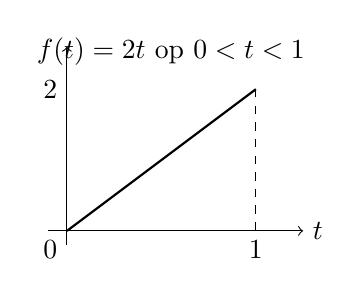
\begin{tikzpicture}[x=2.4cm,y=0.9cm]
\draw[->] (-0.1,0) -- (1.25,0) node[right] {$t$};
\draw[->] (0,-0.2) -- (0,2.6) node[above] {};
\node[below left] at (0,0) {0};
\draw[thick] (0,0) -- (1,2);
\draw[dashed] (1,2) -- (1,0);
\node[below] at (1,0) {1};
\node[left] at (0,2) {2};
\node[above] at (0.55,2.2) {$f(t)=2t$ op $0<t<1$};
\end{tikzpicture}
\end{center}

\textbf{Vraag:}
\begin{enumerate}[label=(\alph*)]
\item Bereken $a_0$.
\item Bepaal $b_1$ en $b_2$.
\item Schrijf de benaderende Fouriersom met 2 termen.
\end{enumerate}

\subsection{Oefening 5.3: Driehoekgolf}

Een driehoekgolf met periode $T = 2$ is gedefinieerd als:
\[
f(t) = \begin{cases}
t, & 0 \le t < 1 \\
2-t, & 1 \le t < 2
\end{cases}
\]

\textbf{Vraag:}
\begin{enumerate}[label=(\alph*)]
\item Is dit signaal even of oneven?
\item Bepaal de Fouriercoëfficiënten.
\item Schrijf de eerste drie niet-nul termen van de Fourierreeks.
\end{enumerate}

\subsection{Oefening 5.4: Parseval's Stelling voor Fourierreeksen}

Gegeven de blokgolf uit oefening 5.1.

\textbf{Vraag:}
\begin{enumerate}[label=(\alph*)]
\item Bereken de gemiddelde macht van het signaal: $P = \frac{1}{T}\int_0^T f^2(t) dt$.
\item Bereken $P$ uit de Fouriercoëfficiënten met Parseval's stelling: $P = a_0^2 + \frac{1}{2}\sum_{n=1}^{\infty} (a_n^2 + b_n^2)$.
\item Controleer dat beide methoden dezelfde waarde geven.
\end{enumerate}

\subsection{Oefening 5.5: Complexe Fourierreeks en Link met FTC}

Definieer een periodiek signaal met periode $T=2$ als
\[
f(t) = \begin{cases}
1, & 0 < t < 1 \\
0, & 1 < t < 2
\end{cases}
\quad \text{en periodiek uitgebreid.}
\]

\textbf{Vraag:}
\begin{enumerate}[label=(\alph*)]
\item Bepaal de complexe Fouriercoëfficiënten $c_k$ (met $\omega_0 = 2\pi/T$).
\item Geef een eenvoudige interpretatie van welke harmonischen verdwijnen.
\item Gebruik de link uit het formularium $X(k\omega_0)=T\,c_k$ om uit te leggen hoe de FTC van \emph{één periode} gesampled wordt.
\end{enumerate}

\subsection{Oefening 5.6: Fourierreeks van een eenvoudige som}

Neem een periodiek signaal met periode $T=2\pi$:
\[
f(t)=\sin(t)+2\cos(2t).
\]

\textbf{Vraag:}
\begin{enumerate}[label=(\alph*)]
\item Geef $\omega_0$.
\item Bepaal de reële Fouriercoëfficiënten $a_0$, $a_n$ en $b_n$.
\item Schrijf de Fourierreeks expliciet (je mag meteen herkennen welke termen niet nul zijn).
\end{enumerate}

\newpage

\section{Hoofdstuk 6: LTC-Systemen}

\subsection{Oefening 6.1: Impulsrespons}

Een eerste-orde systeem heeft impulsrespons $h(t) = 2e^{-5t}u(t)$.

\begin{center}
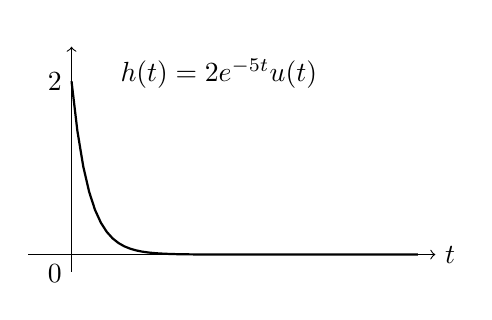
\begin{tikzpicture}[x=1.1cm,y=1.1cm]
\draw[->] (-0.5,0) -- (4.2,0) node[right] {$t$};
\draw[->] (0,-0.2) -- (0,2.4) node[above] {};
\node[below left] at (0,0) {0};
\draw[thick,domain=0:4,samples=60] plot (\x,{2*exp(-5*\x)});
\node[above] at (1.7,1.8) {$h(t)=2e^{-5t}u(t)$};
\node[left] at (0,2) {2};
\end{tikzpicture}
\end{center}

\textbf{Vraag:}
\begin{enumerate}[label=(\alph*)]
\item Bereken de systeemrespons op een stapingang $f(t) = u(t)$ door convolutie.
\item Verifieer je antwoord met de Laplacetransformatie.
\end{enumerate}

\subsection{Oefening 6.2: Massa-Veer-Demper}

Een massa-veer-dempersysteem heeft $m = 2$ kg, $k = 8$ N/m, en $c = 4$ Ns/m.

\textbf{Vraag:}
\begin{enumerate}[label=(\alph*)]
\item Schrijf de differentiaalvergelijking.
\item Bepaal de natuurlijke eigenfrequentie $\omega_0$.
\item Is het systeem ondergedempt, kritisch gedempt, of overgedempt?
\end{enumerate}

\subsection{Oefening 6.3: Frequentierespons}

Gegeven een LTC-systeem met overdracht $H(s) = \frac{10}{s+5}$.

\textbf{Vraag:}
\begin{enumerate}[label=(\alph*)]
\item Bepaal de frequentierespons $H(j\omega)$.
\item Bepaal de amplitude- en faserespons.
\item Bepaal de 3dB bandbreedte (waar $|H(j\omega)| = \frac{|H(0)|}{\sqrt{2}}$).
\end{enumerate}

\subsection{Oefening 6.4: Cascade Systemen}

Gegeven twee LTC-systemen in cascade:
\[
H_1(s) = \frac{5}{s+2}, \quad H_2(s) = \frac{3}{s+3}
\]

\textbf{Vraag:}
\begin{enumerate}[label=(\alph*)]
\item Bepaal de totale overdracht $H(s) = H_1(s) \cdot H_2(s)$.
\item Bepaal de impulsrespons $h(t) = \mathcal{L}^{-1}\{H(s)\}$.
\end{enumerate}

\subsection{Oefening 6.5: Stabiliteit en Polen}

Bepaal voor de volgende systemen of ze BIBO-stabiel, marginaal stabiel of onstabiel zijn op basis van hun polen.

\textbf{Vraag:}
\begin{enumerate}[label=(\alph*)]
\item $H_1(s) = \frac{1}{s-2}$
\item $H_2(s) = \frac{1}{s^2+3s+2}$
\item $H_3(s) = \frac{1}{s^2+4}$
\end{enumerate}

\subsection{Oefening 6.6: Overdracht, Impulsrespons en Nultoestandsrespons}

Een LTC-systeem voldoet aan de differentiaalvergelijking (met nul beginvoorwaarden)
\[
\frac{dy}{dt} + 3y(t) = x(t).
\]

\textbf{Vraag:}
\begin{enumerate}[label=(\alph*)]
\item Bepaal de overdrachtsfunctie $H(s)=\frac{Y(s)}{X(s)}$.
\item Bepaal de impulsrespons $h(t)$.
\item Is het systeem BIBO-stabiel? Motiveer via de polen.
\item Bepaal de nultoestandsrespons $y(t)$ voor $x(t)=u(t)-u(t-1)$.
\end{enumerate}

\subsection{Oefening 6.7: Impuls- en staprespons (basis)}

Een causaal LTC-systeem heeft overdracht
\[
H(s)=\frac{1}{s+1}.
\]

\textbf{Vraag:}
\begin{enumerate}[label=(\alph*)]
\item Bepaal de impulsrespons $h(t)$.
\item Bepaal de staprespons $y(t)$ voor $x(t)=u(t)$.
\item Wat is de tijdsconstante $\tau$ en de DC-versterking $H(0)$?
\end{enumerate}

\newpage

\section{Hoofdstuk 7: Eigenwaarden en Eigenvectoren}

\subsection{Oefening 7.1: Eigenwaarden Berekenen}

Gegeven de matrix:
\[
A = \begin{pmatrix} 4 & 1 \\ 2 & 3 \end{pmatrix}
\]

\textbf{Vraag:}
\begin{enumerate}[label=(\alph*)]
\item Bepaal de karakteristieke veelterm $f(\lambda) = |A - \lambda I|$.
\item Vind de eigenwaarden van $A$.
\item Bereken voor elke eigenwaarde een bijbehorende eigenvector.
\end{enumerate}

\subsection{Oefening 7.2: Eigenwaarden van Tweede-Orde Systeem}

Voor het systeem uit oefening 3.4 ($\frac{d^2y}{dt^2} + 4\frac{dy}{dt} + 3y = 0$).

\textbf{Vraag:}
\begin{enumerate}[label=(\alph*)]
\item Schrijf dit differentiaalvergelijkingssysteem als een eerste-orde matrixvergelijking:
\[
\frac{d}{dt}\begin{pmatrix} y \\ \dot{y} \end{pmatrix} = \begin{pmatrix} 0 & 1 \\ -3 & -4 \end{pmatrix} \begin{pmatrix} y \\ \dot{y} \end{pmatrix}
\]
\item Bepaal de eigenwaarden van deze systeemmatrix.
\item Verifieer dat dit overeenkomt met de karakteristieke vergelijking uit oefening 3.4.
\item Bepaal de eigenvectoren.
\end{enumerate}

\subsection{Oefening 7.3: Diagonalisatie}

Gegeven de matrix:
\[
A = \begin{pmatrix} 5 & -2 \\ -2 & 2 \end{pmatrix}
\]

\textbf{Vraag:}
\begin{enumerate}[label=(\alph*)]
\item Bepaal alle eigenwaarden en bijbehorende eigenvectoren.
\item Controleer dat de eigenvectoren orthogonaal zijn (omdat $A$ symmetrisch is).
\item Vorm de matrix $P$ met eigenvectoren als kolommen en bepaal $P^{-1}AP = D$ waarbij $D$ diagonaal is.
\end{enumerate}

\subsection{Oefening 7.4: Gerschgorin-Cirkelstelling}

Gegeven de matrix:
\[
A = \begin{pmatrix} 4 & 0.5 & 0.2 \\ 0.3 & -2 & 0.1 \\ 0.2 & 0.4 & 3 \end{pmatrix}
\]

\textbf{Vraag:}
\begin{enumerate}[label=(\alph*)]
\item Bepaal de Gerschgorin-cirkels voor deze matrix.
\item Geef grenzen voor de eigenwaarden op basis van de stelling.
\item Bepaal de eigenwaarden numeriek en controleer of ze binnen de cirkels vallen.
\end{enumerate}

\subsection{Oefening 7.5: Eigenvectoren en Orthogonaliteit}

Gegeven de matrix:
\[
B = \begin{pmatrix} 3 & 1 \\ 1 & 3 \end{pmatrix}
\]

\textbf{Vraag:}
\begin{enumerate}[label=(\alph*)]
\item Bepaal de eigenwaarden.
\item Bepaal de eigenvectoren.
\item Toon aan dat de eigenvectoren orthogonaal zijn.
\item Normaliseer de eigenvectoren tot eenheid.
\end{enumerate}

\subsection{Oefening 7.6: Matrix Exponentiële}

Gegeven de matrix $A = \begin{pmatrix} 0 & 1 \\ -2 & -3 \end{pmatrix}$.

\textbf{Vraag:}
\begin{enumerate}[label=(\alph*)]
\item Bepaal de eigenwaarden en eigenvectoren van $A$.
\item Bereken de matrix exponentiële $e^{At}$ via diagonalisatie of Cayley-Hamilton.
\item Gebruik dit om de oplossing van $\dot{\mathbf{x}} = A\mathbf{x}$ te vinden met $\mathbf{x}(0) = \begin{pmatrix} 1 \\ 0 \end{pmatrix}$.
\end{enumerate}

\subsection{Oefening 7.7: Niet-diagonaliseerbaar en Matrixexponentiaal}

Gegeven
\[
A = \begin{pmatrix} 2 & 1 \\ 0 & 2 \end{pmatrix}.
\]

\textbf{Vraag:}
\begin{enumerate}[label=(\alph*)]
\item Bepaal de eigenwaarden van $A$ en de dimensie van de eigenruimte.
\item Is $A$ diagonaliseerbaar? Motiveer.
\item Bepaal $e^{At}$.
\end{enumerate}

\subsection{Oefening 7.8: Eigenwaarden van een diagonaalmatrix (basis)}

Gegeven
\[
A=\begin{pmatrix}1 & 0\\ 0 & 2\end{pmatrix}.
\]

\textbf{Vraag:}
\begin{enumerate}[label=(\alph*)]
\item Bepaal de eigenwaarden en geef voor elke eigenwaarde een eigenvector.
\item Bereken $A^3$.
\item Bereken $e^{At}$.
\end{enumerate}

\newpage

\section{Hoofdstuk 8: Examengerichte Oefeningen}

\subsection{Oefening 8.1: FTC-eigenschappen (Verschuiving en Modulatie)}

Definieer het bloksignaal
\[
x(t) = \begin{cases}
1, & -\tfrac{1}{2}<t<\tfrac{1}{2}\\
0, & \text{elsewhere}
\end{cases}
\]
en de cosinus $v(t)=2\cos(2\pi t)$. Definieer $y(t)=x(t)\cos(2\pi t)$ en $z(t)=x(t)+x(t-1)$.

\textbf{Vraag:}
\begin{enumerate}[label=(\alph*)]
\item Welke van de signalen $x(t)$, $v(t)$, $y(t)$ en $z(t)$ zijn even/oneven?
\item Bepaal $Y(j\omega)$ met de modulatiestelling en een gekende FTC-paar voor $x(t)$.
\item Bepaal $Z(j\omega)$ met de verschuivingsstelling.
\end{enumerate}

\subsection{Oefening 8.2: Laplace, Causaliteit en Convolutie}

Het ingangssignaal is $x(t)=u(t)-u(t-2)$ en de impulsrespons is $h(t)=e^{-t}u(t)$.

\begin{center}
\begin{tikzpicture}[x=1.0cm,y=1.0cm]
\draw[->] (-0.5,0) -- (4.2,0) node[right] {$t$};
\draw[->] (0,-0.2) -- (0,1.6) node[above] {};
\node[below left] at (0,0) {0};
% x(t)
\draw[thick] (0,0) -- (0,1) -- (2,1) -- (2,0);
\node[above] at (1,1) {$x(t)$};
\node[below] at (2,0) {2};
\end{tikzpicture}
\end{center}

\textbf{Vraag:}
\begin{enumerate}[label=(\alph*)]
\item Bepaal $X(s)$.
\item Is het systeem causaal? Motiveer op basis van $h(t)$.
\item Bepaal $y(t)=h(t)*x(t)$ en geef het antwoord stukgewijs.
\end{enumerate}

\subsection{Oefening 8.3: Complexe Fourierreeks (Puls-trein)}

Definieer een periodiek signaal met periode $T=2$ als
\[
p(t)=\begin{cases}
1, & 0<t<\tfrac{1}{2}\\
0, & \tfrac{1}{2}<t<2
\end{cases}
\quad \text{en periodiek uitgebreid.}
\]

\textbf{Vraag:}
\begin{enumerate}[label=(\alph*)]
\item Bepaal de complexe Fouriercoëfficiënten $c_k$.
\item Welke symmetrie zie je in $c_{-k}$ t.o.v. $c_k$ als $p(t)$ reëel is?
\item (Extra) Gebruik opnieuw de link $X(k\omega_0)=T\,c_k$ om te interpreteren wat de harmonischen betekenen in het frequentiedomein.
\end{enumerate}

\subsection{Oefening 8.4: Laplace met verschuiving en initieelwaarden}

Beschouw
\[
x(t)=e^{-t}u(t)-e^{-(t-2)}u(t-2).
\]

\textbf{Vraag:}
\begin{enumerate}[label=(\alph*)]
\item Bepaal $X(s)$.
\item Bepaal $x(0^+)$ en $\lim_{t\to\infty}x(t)$ rechtstreeks uit $x(t)$.
\item Verifieer $x(0^+)$ met de beginwaardestelling en $\lim_{t\to\infty}x(t)$ met de eindwaardestelling (als toepasbaar).
\end{enumerate}

\subsection{Oefening 8.5: Differentiaalvergelijking (Laplace, stapinput)}

Gegeven
\[
y''(t)+3y'(t)+2y(t)=u(t),\qquad y(0)=0,\quad y'(0)=1.
\]

\textbf{Vraag:}
\begin{enumerate}[label=(\alph*)]
\item Los $y(t)$ op met de (unilaterale) Laplace-transformatie.
\item Geef $y(t)$ stukgewijs (indien nodig) en vereenvoudig maximaal.
\end{enumerate}

\subsection{Oefening 8.6: LTI-systeem (polen, stabiliteit, staprespons)}

Een causaal LTI-systeem heeft
\[
H(s)=\frac{s+2}{s(s+4)}.
\]

\textbf{Vraag:}
\begin{enumerate}[label=(\alph*)]
\item Bepaal $h(t)$.
\item Is het systeem BIBO-stabiel? Motiveer.
\item Bepaal de staprespons $y(t)$ voor $x(t)=u(t)$.
\item Bepaal $\lim_{t\to\infty}y(t)$ en controleer met de eindwaardestelling.
\end{enumerate}

\subsection{Oefening 8.7: Convolutie + Laplace-check}

Neem $x(t)=u(t)-u(t-1)$ en $h(t)=t\,u(t)$.

\textbf{Vraag:}
\begin{enumerate}[label=(\alph*)]
\item Bepaal $y(t)=(x*h)(t)$ via convolutie in het tijdsdomein en geef het resultaat stukgewijs.
\item Controleer je antwoord door Laplace: $Y(s)=X(s)H(s)$ en inverse Laplace.
\end{enumerate}

\subsection{Oefening 8.8: Fouriertransformatie + Parseval (energie)}

Voor $a>0$:
\[
x(t)=e^{-a|t|}.
\]

\textbf{Vraag:}
\begin{enumerate}[label=(\alph*)]
\item Bepaal $X(j\omega)$.
\item Bereken de energie $E=\int_{-\infty}^{\infty}|x(t)|^2\,dt$.
\item Controleer met Parseval.
\end{enumerate}

\subsection{Oefening 8.9: Reële Fourierreeks (symmetrie + RMS)}

Definieer een periodiek signaal met periode $T=2\pi$:
\[
f(t)=\begin{cases}
1, & 0<t<\pi\\
-1, & -\pi<t<0
\end{cases}
\quad \text{en periodiek uitgebreid.}
\]

\textbf{Vraag:}
\begin{enumerate}[label=(\alph*)]
\item Geef aan of $f(t)$ even/oneven is.
\item Bepaal de reële Fourierreeks van $f(t)$.
\item Bepaal de RMS-waarde van $f(t)$ en verifieer met Parseval (reeks-vorm).
\end{enumerate}

\subsection{Oefening 8.10: Toestandruimte en eigenwaarden (stabiliteit + oplossing)}

Beschouw het systeem
\[
\dot{\mathbf{x}}=A\mathbf{x},\qquad
A=\begin{pmatrix}0 & 1\\ -2 & -3\end{pmatrix},\qquad \mathbf{x}(0)=\begin{pmatrix}1\\0\end{pmatrix}.
\]

\textbf{Vraag:}
\begin{enumerate}[label=(\alph*)]
\item Bepaal de eigenwaarden van $A$ en bespreek de stabiliteit van de oorsprong.
\item Bepaal $\mathbf{x}(t)$ expliciet (via diagonalisatie of via oplossing van een tweede-orde vergelijking).
\item Geef ook $x_1(t)$ en $x_2(t)$ afzonderlijk.
\end{enumerate}

\subsection{Oefening 8.11: Impulsrespons en Stabiliteit met Polen}

Gegeven een causaal LTC-systeem met overdrachtsfunctie
\[
H(s) = \frac{2s + 3}{s^2 + 5s + 6}.
\]

\emph{Bron: Oefeningenbundel 25–26 (thema Laplace en LTI-systemen).}

\textbf{Vraag:}
\begin{enumerate}[label=(\alph*)]
\item Bepaal de polen van het systeem.
\item Onderzoek BIBO-stabiliteit op basis van de poollocaties.
\item Bepaal de impulsrespons $h(t) = \mathcal{L}^{-1}\{H(s)\}$ via partieelbreuken.
\item Bepaal de staprespons voor $x(t) = u(t)$.
\end{enumerate}

\subsection{Oefening 8.12: Differentiaalvergelijking uit Overdrachtsfunctie}

Een LTC-systeem wordt beschreven door de overdrachtsfunctie
\[
H(s) = \frac{Y(s)}{X(s)} = \frac{4}{s^2 + 3s + 2}.
\]

\emph{Bron: Oefeningenbundel 25–26 (thema differentiaalvergelijkingen en Laplace).}

\textbf{Vraag:}
\begin{enumerate}[label=(\alph*)]
\item Bepaal de differentiaalvergelijking die het systeem beschrijft.
\item Los deze differentiaalvergelijking op (homogeen + particulier) voor input $x(t) = 2u(t)$ met beginvoorwaarden $y(0) = 0$ en $y'(0) = 1$.
\item Controleer je antwoord met de Laplacetransformatie.
\end{enumerate}

\subsection{Oefening 8.13: Fouriertransformatie van Exponentieel Signaal}

Gegeven het signaal
\[
f(t) = 3e^{-2t}u(t).
\]

\emph{Bron: Oefeningenbundel 25–26 (Fouriertransformatie en energieanalyse).}

\textbf{Vraag:}
\begin{enumerate}[label=(\alph*)]
\item Bepaal de Fouriertransformatie $F(j\omega)$ (gebruik de link met Laplace).
\item Bepaal en schets het amplitudespectrum $|F(j\omega)|$.
\item Bereken de energiedichtheid $E = \int_{-\infty}^{\infty} |f(t)|^2 dt$.
\item Verifieer Parseval's stelling: $E = \frac{1}{2\pi}\int_{-\infty}^{\infty} |F(j\omega)|^2 d\omega$.
\end{enumerate}

\newpage

\section{Oplossingen}

\subsection{Oplossingen Hoofdstuk 1}

\subsubsection*{Oplossing 1.1}

\textbf{Gegeven:} Systeem met operator $\mathcal{T}\{x(t)\} = 3x(t) + 2$.

\textbf{Vraag:} Onderzoek of dit systeem lineair is.

\textbf{Oplossing:}

\begin{itemize}
\item Test eigenschap 1 (schaling): $\mathcal{T}\{ax(t)\} = 3ax(t) + 2 \neq a\mathcal{T}\{x(t)\} = a(3x(t) + 2) = 3ax(t) + 2a$
\item Voor $a \neq 1$ geldt: $2 \neq 2a$, dus schaling klopt niet.
\item Omdat de schalingsvoorwaarde niet voldaan is, is het systeem niet lineair.
\end{itemize}

\subsubsection*{Oplossing 1.2}

\textbf{Gegeven:} RC-circuit met $R = 1000$ $\Omega$, $C = 10$ $\mu$F, ingangsspanning $v_{\text{in}}(t) = 5u(t)$ V.

\textbf{Vraag:} 
\begin{enumerate}[label=(\alph*)]
\item Schrijf de differentiaalvergelijking op.
\item Bereken $\tau$.
\item Bepaal $v_{\text{uit}}(0.01)$.
\end{enumerate}

\textbf{Oplossing:}

\begin{enumerate}[label=(\alph*)]
\item De differentiaalvergelijking van een RC-circuit: $RC\frac{dv_{\text{uit}}}{dt} + v_{\text{uit}} = v_{\text{in}}$

\[
(1000)(10 \times 10^{-6})\frac{dv_{\text{uit}}}{dt} + v_{\text{uit}} = 5u(t)
\]

\[
0.01\frac{dv_{\text{uit}}}{dt} + v_{\text{uit}} = 5u(t)
\]

\item Tijdsconstante: $\tau = RC = (1000)(10 \times 10^{-6}) = 0.01$ s $= 10$ ms

\item Voor een staprespons met $v_{\text{uit}}(0) = 0$:

\[
v_{\text{uit}}(t) = 5(1 - e^{-t/\tau})u(t) = 5(1 - e^{-100t})u(t)
\]

Op $t = 10$ ms $= 0.01$ s:

\[
v_{\text{uit}}(0.01) = 5(1 - e^{-1}) = 5(1 - 0.368) = 5(0.632) = 3.16 \text{ V}
\]
\end{enumerate}

\subsubsection*{Oplossing 1.3}

\textbf{Gegeven:} Radio-isotoop met halveringstijd $t_{1/2} = 6$ uur. Initiële hoeveelheid: 20 mg om 08:00.

\textbf{Vraag:} Hoeveel mg blijft over om 14:00?

\textbf{Oplossing:}

Model radioactief verval: $N(t) = N_0 e^{-kt}$

Halveringstijd $t_{1/2} = 6$ uur: $\frac{1}{2} = e^{-6k} \Rightarrow k = \frac{\ln(2)}{6} = 0.1155$ h$^{-1}$

Van 08:00 tot 14:00 is $\Delta t = 6$ uur:

\[
N(6) = 20 e^{-0.1155 \times 6} = 20 e^{-0.693} = 20 \times 0.5 = 10 \text{ mg}
\]

\textbf{Antwoord:} 10 mg blijft over.

\subsubsection*{Oplossing 1.4}

\textbf{Gegeven:} Twee systemen:
- Systeem A: $\mathcal{T}\{x(t)\} = 2x(t)$
- Systeem B: $\mathcal{T}\{x(t)\} = x(t) + 1$

\textbf{Vraag:} Test op homogeniteit en additiviteit; bepaal lineariteit.

\textbf{Oplossing:}

\textbf{Systeem A: } $\mathcal{T}\{x(t)\} = 2x(t)$

Homogeniteit: $\mathcal{T}\{ax(t)\} = 2ax(t) = a(2x(t)) = a\mathcal{T}\{x(t)\}$ \checkmark

Additiviteit: $\mathcal{T}\{x_1(t) + x_2(t)\} = 2(x_1(t) + x_2(t)) = 2x_1(t) + 2x_2(t) = \mathcal{T}\{x_1(t)\} + \mathcal{T}\{x_2(t)\}$ \checkmark

\textbf{Systeem A is LINEAIR.}

\textbf{Systeem B: } $\mathcal{T}\{x(t)\} = x(t) + 1$

Homogeniteit: $\mathcal{T}\{ax(t)\} = ax(t) + 1 \neq a(x(t) + 1) = ax(t) + a = a\mathcal{T}\{x(t)\}$ (voor $a \neq 1$) \text{\sffamily X}

\textbf{Systeem B is NIET LINEAIR.}

\subsubsection*{Oplossing 1.5}

\textbf{Gegeven:} Vier systemen. 
\textbf{Vraag:} Welke zijn LTI?

\textbf{Oplossing:}

\begin{enumerate}[label=(\alph*)]
\item $y(t) = x(t-2)$: LINEAIR en TIJDINVARIANT \checkmark (zuivere vertraging)

\item $y(t) = tx(t)$: LINEAIR maar NIET TIJDINVARIANT \text{\sffamily X} (coëfficiënt varieert in tijd)

\item $y(t) = |x(t)|$: NIET LINEAIR \text{\sffamily X} (niet additief/homogeen)

\item $y(t) = \int_0^t x(\tau) d\tau$: LINEAIR en TIJDINVARIANT \checkmark (integrator)

\end{enumerate}

\textbf{Antwoord:} (a) en (d) zijn LTI.

\subsubsection*{Oplossing 1.6}

\textbf{Gegeven:} $y(t)=x(t)+x(t-1)$.

\textbf{Vraag:} Onderzoek lineariteit/tijdinvariantie; causaliteit; invertibiliteit.

\textbf{Oplossing:}
\begin{enumerate}[label=(\alph*)]
\item \textbf{Lineair en tijdinvariant:} Het systeem is lineair (som van lineaire operatoren) en tijdinvariant omdat een tijdsverschuiving van de input dezelfde verschuiving in beide termen geeft.
\item \textbf{Causaal:} Ja. $y(t)$ hangt af van $x(t)$ en $x(t-1)$, dus enkel van huidige en verleden waarden.
\item \textbf{Invertibel:} \textbf{Niet} uniek invertibel.

\textbf{Bewijs door tegenvoorbeeld:}

Stel $y(t) = 0$ voor alle $t$. Dan geldt:
\[
x(t) + x(t-1) = 0 \Rightarrow x(t) = -x(t-1)
\]

Deze vergelijking heeft oneindig veel oplossingen, bijvoorbeeld:
\begin{itemize}
\item $x(t) = A(-1)^t$ voor elke constante $A$
\item $x(t) = 0$ voor alle $t$
\end{itemize}

Omdat verschillende inputs tot dezelfde output leiden, is het systeem niet invertibel.
\end{enumerate}

\subsubsection*{Oplossing 1.7}

\textbf{Gegeven:} (S1) $y(t)=2x(t-1)$ en (S2) $y(t)=x(t)+u(t)$.

\textbf{Vraag:} Onderzoek lineariteit, tijdinvariantie en causaliteit voor (S1) en (S2).

\textbf{Oplossing:}

\begin{enumerate}[label=(\alph*)]
\item \textbf{Lineariteit}

\textbf{Systeem (S1): $y(t)=2x(t-1)$}

\textbf{Test homogeniteit:} Voor $ax(t)$:
\[
\mathcal{T}\{ax(t)\} = 2ax(t-1) = a\cdot 2x(t-1) = a\mathcal{T}\{x(t)\} \quad \checkmark
\]

\textbf{Test additiviteit:} Voor $x_1(t) + x_2(t)$:
\[
\mathcal{T}\{x_1(t)+x_2(t)\} = 2(x_1(t-1)+x_2(t-1)) = 2x_1(t-1) + 2x_2(t-1) = \mathcal{T}\{x_1(t)\} + \mathcal{T}\{x_2(t)\} \quad \checkmark
\]

$\Rightarrow$ (S1) is \textbf{lineair}.

\textbf{Systeem (S2): $y(t)=x(t)+u(t)$}

\textbf{Nultoestandtest:} Voor $x(t)=0$:
\[
\mathcal{T}\{0\} = 0 + u(t) = u(t) \neq 0
\]

Dit schendt het nultoestandcriterium voor lineariteit.

$\Rightarrow$ (S2) is \textbf{niet lineair}.

\item \textbf{Tijdinvariantie}
\begin{itemize}
\item (S1) is \textbf{tijdinvariant}: $x(t)\mapsto x(t-t_0)$ geeft $y(t)=2x(t-1)\mapsto 2x(t-t_0-1)=y(t-t_0)$.
\item (S2) is \textbf{niet tijdinvariant}: voor $x(t)$ is $y(t)=x(t)+u(t)$. Voor $x(t-t_0)$ is de output $x(t-t_0)+u(t)$, terwijl $y(t-t_0)=x(t-t_0)+u(t-t_0)$. Niet gelijk als $t_0\neq 0$.
\end{itemize}

\item \textbf{Causaliteit}
\begin{itemize}
\item (S1) is \textbf{causaal}: $y(t)$ hangt af van $x(t-1)$ (verleden).
\item (S2) is \textbf{causaal}: $y(t)$ hangt af van $x(t)$ en een gekend signaal $u(t)$.
\end{itemize}
\end{enumerate}

\end{document}